\documentclass[t,10pt,mathserif,xcolor=pst,pdftex]{beamer}
\mode<presentation>

\usetheme{Berkeley}
\usecolortheme{dolphin}
\beamertemplatenavigationsymbolsempty
\usefonttheme[onlylarge]{serif}

\usepackage[USenglish]{babel}
\usepackage[utf8]{inputenc}
\usepackage[T1]{fontenc}
\usepackage{colortbl}
\usepackage{pstricks}
\usepackage{multimedia}
\usepackage{bm}
\usepackage{nicefrac}
\usepackage{charter}
\def\Rz{\mathbb{R}}
\def\Cz{\mathbb{C}}
\newcommand{\be}{\begin{equation}} 
\newcommand{\ee}{\end{equation}}  
\newcommand{\bea}{\begin{eqnarray}}
\newcommand{\eea}{\end{eqnarray}}
\newcommand{\bvec}[1]{\mathbf{#1}}
\newcommand{\transp}{^{\mathrm{T}}}
\newcommand{\brho}{\boldsymbol{\rho}}
\newcommand{\br}{\textbf{r}}
\newcommand{\bq}{\textbf{q}}
\newcommand{\by}{\textbf{y}}
\newcommand{\bz}{\textbf{z}}
\newcommand{\Vavg}{\langle V \rangle_{H'}}
\newcommand{\angstrom}{\mbox{\normalfont\AA}}
\newcommand{\Eq}[1]{Eq.~\eqref{#1}}
\newcommand{\Eqs}[1]{Eqs.~\eqref{#1}}
\newcommand{\Fig}{Fig. \ref}
\newcommand{\Tab}{Table. \ref}

\newcommand{\pd}{\partial}

\title[Chem 132A]{Physical Chemistry (Chem 132A)}

\author[Shane Flynn]{Presentation By: Shane Flynn}
\institute[UC Irvine]{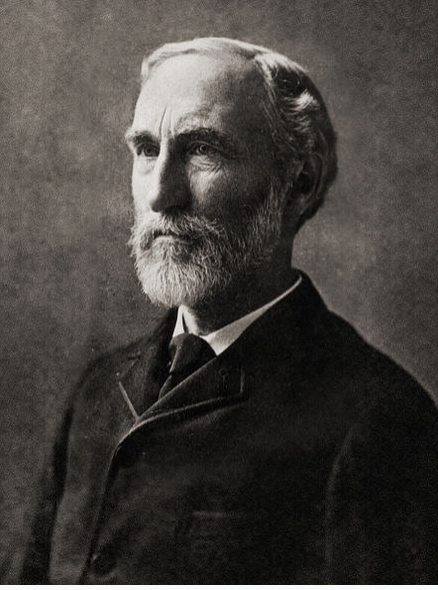
\includegraphics[height=0.40\textheight,width=0.35\textwidth]{Gibbs.png}\\[1mm]
Department of Chemistry, University of California, Irvine, 2208 Natural Sciences II}

\date\today

\pgfdeclareimage[height=1.5cm]{logo}{uc_seal.png}
\logo{\pgfuseimage{logo}}

\begin{document}

\begin{frame}
\titlepage
\end{frame}

\section{What We Know}

\subsection{The First Law}

\begin{frame}{Navigating The Equations}
\begin{itemize}
\item The First Law of Thermodynamics
\end{itemize}
\be
\Delta U = q + w
\ee

\be
w_{PV} = -\int_{V_i}^{V_f}P_{ext}dV
\ee

$\qquad$ {\small{Assume an Equation of State to solve for work! ... q=?, U(T,V)}}

\begin{itemize}
\item State Functions and Total Differentials
\end{itemize}
\be
dU = \left(\frac{\pd U}{\pd T}\right)_VdT + \left(\frac{\pd U}{\pd V}\right)_T dV 
\ee
\begin{itemize}
\item Giving Names to Partial Derivatives
\end{itemize}
\be
C_V \equiv \left(\frac{\pd U}{\pd T}\right)_V \quad \Rightarrow \quad q = C_V\Delta T
\ee
\end{frame}

\subsection{Enthalpy}

\begin{frame}{Navigating The Equations}

\begin{itemize}
\item Different Thermodynamic Potentials
\end{itemize}
\be
H \equiv U + PV
\ee
\begin{itemize}
\item Consider a Different Total Differential H(T,P)
\end{itemize}

\be
C_P \equiv \left(\frac{\pd H}{\pd T}\right)_P
\ee
And using a new set of assumptions we were able to express the heat in a different form. 
\be
q = C_P\Delta T
\ee

\end{frame}

\subsection{The Second Law}

\begin{frame}{Navigating The Equations}
\begin{itemize}
\item Heat and Energy $\cdots$ Chemists Want Direction
\item Enter The Second Law of Thermodynamics
\end{itemize}
\be
dS \equiv \frac{\delta q_r}{T}, \quad \Rightarrow \quad \Delta S = \int_i^f \frac{\delta q_r}{T}
\ee

\begin{itemize}
\item And we claimed without any justification that Entropy was a state function (Integrating Factor). 
\end{itemize}

\begin{itemize}
\item We think of entropy as the 'disorder', and people discuss things like 'number of micro-states'.
\item Take Statistical Mechanics if you would like a more rigorous definition!
\end{itemize}
\be
dS \geq \frac{\delta q}{T}
\ee

\end{frame}

\section{Helmholtz Free Energy}

\begin{frame}{Accounting For Entropy}

\begin{itemize}
\item Perpetual Motion, Maxwell's Demon $\cdots$ No Free Lunch.
\end{itemize}

\begin{itemize}
\item Entropy as the Universal Tax, we MUST account for it.
\end{itemize}

\hfill \break
{\Large{Defining a new Thermodynamic Potential:}} 
\newline
\begin{itemize}
\item Closed system; constant Volume, constant Temperature. 
\end{itemize}
\be
\begin{split}
    dU &= \delta q \\
    dS &\geq \left(\frac{dU}{T}\right)_V\\
    TdS &\geq dU \\
    0 &\geq dU - TdS\\
    0 &\geq d(U - TS)\\
    \end{split}
\ee

\end{frame}

\begin{frame}{The Helmholtz Free Energy}
\begin{itemize}
\item What does this mean and why should we care?
\end{itemize}
\be
A \equiv U - TS
\ee

\begin{itemize}
\item A is called the \textbf{Helmholtz Free Energy}
\end{itemize}

\begin{itemize}
\item All of these variables are in terms of the \textbf{SYSTEM}.
\end{itemize}

\begin{itemize}
\item The derivation assumes constant T and V $\quad \Rightarrow \quad$ A(T,V). 
\end{itemize}

\begin{itemize}
\item  A system with a negative Helmholtz implies a spontaneous process.
\end{itemize}

\be
\Delta A = \Delta U - T\Delta S
\ee

\begin{itemize}
\item  If S is negative, U would have to be negative to be spontaneous; $\qquad$ heat enters the environment.
\end{itemize}

\end{frame}

\subsection{Reversible Work}

\begin{frame}{Helmholtz as the Work Function}
\be
\Delta A = \Delta U - T\Delta S
\ee


\begin{itemize}
\item Clearly we need either negative Internal Energy or positive Entropy, to generate a spontaneous Helmholtz Free Energy.
\end{itemize}

\begin{itemize}
\item Consider a reversible process with constant Temperature.
\end{itemize}
\be
    \begin{split}
        \Delta A_r &= \Delta U_r - T\Delta S_r \\
        &= \Delta U_r - T\frac{q_r}{T} \\
        &= \Delta U_r - q_r \\
        &= q_r + w_r - q_r \\
        \Delta A_r &= w_r
    \end{split}
\ee

\end{frame}

\section{Gibbs Free Energy}

\begin{frame}{Accounting For Entropy $\cdots$ Again}

{\Large{Defining Another Thermodynamic Potential:}} 
\newline
\begin{itemize}
\item Experimentalists would really like a thermodynamic potential with characteristic variables T and P.
\item A(T,V). $\qquad$ Let's try our strategy again!
\end{itemize}

Consider a constant pressure process, and only PV work.  
\begin{equation}
    \delta q = dH 
\end{equation}
Assuming a constant temperature we can use the Second Law
\be
\begin{split}
dS \geq \frac{\delta q}{T} \Rightarrow &dS - \frac{\delta q}{T} \geq 0\\
TdS - dH &\geq 0 \Rightarrow \\
d(H-TS) &\leq 0
\end{split}
\ee

\end{frame}

\begin{frame}{The Gibbs Free Energy}
\be
G \equiv H - TS
\ee

\begin{itemize}
\item G is called the \textbf{Gibbs Free Energy}
\end{itemize}

\begin{itemize}
\item Again we see that a spontaneous process must have a negative Gibbs Free Energy.  $\qquad \Rightarrow \quad$ G(T,P). 
\end{itemize}

\be
\Delta G = \Delta H - T\Delta S
\ee

\begin{itemize}
\item  If $\Delta$ G = 0, a chemical reaction has no drive to move towards products or reactants. This is equilibrium!
\end{itemize}

{\large{Gibbs: Maximum Non-Expansion Work}}

If you assume constant Temperature, constant Pressure, and a reversible process you find (Page 135).
\be
dG = \delta w_{\text{non-PV}}
\ee

\end{frame}

\section{Conclusion}

\begin{frame}{Summary}
\begin{itemize}
\item We are developing various equations for different sets of physical conditions.
\item The method for developing each set of equations is VERY similar, and depends on what variables you wish to hold constant. 
\item Entropy defines spontaneity. There is no way to avoid The Second Law.
\item The Free Energies (Helmholtz and Gibbs) account for the entropy by construction. 
\item The Free Energies are in terms of the \textbf{SYSTEM}.
\item These potentials are naturally functions of: $\quad$ $\qquad$ $\qquad$ A(T,V) G(T,P)
\end{itemize}
\end{frame}

\end{document}